

\chapter{Prediction of Multi-episodic Judgments}\label{chap:modeling}
An initial approach on the prediction of multi\-/episodic judgments has been conducted by \citet{moller_single-call_2011}.
The model\footnote{The term \emph{model} is used in the following in terms of curve fitting. A model is here a mathematical function, which might be parameterizable, that maps an input space to an output space.} proposed here is to average all \emph{prior} episodic judgments to predict a multi\-/episodic judgment.
\citet{moller_single-call_2011} evaluated the precision of this predictor with their 14~day experiment (\cf{} \autoref{prior:moeller}).
Instead of evaluating the prediction accuracy for \ac{MOS}, the prediction accuracy for each individual participant was evaluated for all three multi\-/episodic judgments taken in this experiment.
Here, multi\-/episodic judgments were taken after the 2nd, 7th, and 14th~day.
With regard to the five conducted multi\-/episodic conditions, it could be shown that the predictor is precise for the 2nd~day and precision decreases for later multi\-/episodic judgments.

This chapter starts with an overview of the effects observed in the here presented experiments that seem relevant for the prediction of multi\-/episodic judgments.
Subsequently, model types are presented that seem suited for the prediction.
The prediction accuracy for these model types is evaluated using only \E1{}, \EIIa{}, and \E6{}.
These experiments yielded large and in itself consistent data sets.\footnote{An approach towards modeling based on the experiment of \citet{moller_single-call_2011} and \E5{} is published in \citet{guse_modelling_2014}. However, these two experiments are omitted here for the development of prediction models due to the limited effects on multi\-/episodic judgments.}
The other here presented experiments (\EIIb{}, \E3{}, \E4{}, and \E5{}) are not considered suitable for the implementation of a prediction model, as only a very limited set of conditions was investigated.
In difference to \citet{moller_single-call_2011}, who predicted multi\-/episodic judgments using episodic judgments per individual participant, the goal is here the prediction of the multi\-/episodic \ac{MOS} based on the episodic \ac{MOS}.
Predicting individual judgments might be desirable, but the conducted experiments did not collect sufficient data to be able to explain differences between individual participants.
In fact, the defined\-/use method was applied, so a \ac{MOS} could be derived that reflects the judgment of the \emph{average actor}.

The here presented modeling is necessarily limited to the development of best fitting predictor(s), as no data sets for cross\-/validation were available.
Furthermore, the conducted experiments differ in the experimental design and also observed effects.
Thus, models created for one experiment cannot be verified validly using data from the other experiments.

\section{Effects on Multi-episodic Judgments}
In the conducted experiments, several effects have been observed.
First, it must be noted that multi\-/episodic judgments are very similar to episodic judgments if no degraded episodes are presented.
This has been observed by \citet{moller_single-call_2011} and also in the here presented experiments.
If no \ac{LP} episodes were presented, the experiment of \citet{moller_single-call_2011} and \E4{} indicated a slight increase of episodic judgments from the first to the last episode in a multi\-/episodic condition.
However, the indicated effect is rather small and the actual reason for this could not be deduced.
It is thus not considered for the implementation of a prediction model.

%\paragraph*{Number of degraded Episodes}
The largest observed effect on multi\-/episodic judgments is the decrease due to an increased number of \ac{LP} usage episodes (\autoref{hypo:number}).
This has been investigated in \E1{}, \EIIa{}, and \E6{}.
Here, a decrease is observed until saturation occurred, \ie, the multi\-/episodic judgment did not decrease further (saturation effect).
This occurred if more than two \ac{LP} episodes/days were presented.
In fact, the final multi\-/episodic judgment remained above the episodic judgments of \ac{LP}.
This shows that the final multi\-/episodic judgment is still affected by previous \ac{HP} episodes, \ie, the integration interval is longer than 3~episodes or 3~days, respectively.
In addition to the integration interval, this indicates that one or all of the three \ac{LP} episodes/days had a reduced impact on the final multi\-/episodic judgment.

In addition, a position effect has been observed (\autoref{hypo:position}).
This has been investigated in \E1{}, \EIIa{}, and \E6{}.
An impact of position and thus a recency effect could be observed in \E1{} and \EIIa{}.
Here, the impact of \ac{LP} episode(s) on the following multi\-/episodic judgment decreased the more \ac{HP} episodes were presented afterwards.
While \E1{} showed such an effect in both cases, \ie, for one and two \ac{LP} episodes, it was only present in \EIIa{} for two \ac{LP} episodes.
This might be attributed to the passive usage situation.
In \E1{}, a two-party conversation was used, whereas \EIIa{} applied a third-party listening task.
Although not statistically significant, a recency effect was indicated in \E6{} for both cases, \ie, one or two days presented in \ac{LP}.

In \EIIa{} and \E6{}, the impact of non\-/consecutive \ac{LP} presentation was also investigated (\autoref{hypo:consecutive}).
An effect could not be observed in both experiments and thus the number of performance changes is assumed to be neglectable for the prediction of multi\-/episodic judgments.
In fact, the small, potential difference might also be explainable by a recency effect.

A peak effect is not considered for modeling, as such an effect could not be observed in \E1{} (\autoref{hypo:strength}).
Even if in \C7{} a peak effect occurred, the influence on the multi\-/episodic judgment seems to be rather small.

For one session, also the recovery of negatively affected multi\-/episodic judgments was investigated (\autoref{hypo:recovery}).
%Here, additional \ac{HP} episodes are presented after a negatively affected multi\-/episodic judgment and the improvement assessed.
This was studied with two conditions in \E1{}.
Here, 9 episodes were presented while non-\ac{HP} episodes were presented as the 5th and the 6th~episode.
The multi\-/episodic judgment after the 6th~episode showed a negative effect, and the judgments after the 3rd and 9th~episode were significantly different.
Thus, in both conditions a negative impact is still present in the final multi\-/episodic judgment.
This finding can be explained by a recency effect or by the increased number of \ac{HP} episodes.

For one session, a duration neglect was investigated in \E3{} (\autoref{hypo:duration}). 
Here, doubling the duration of one \ac{LP} episode did not negatively affect the following multi\-/episodic judgment.
In fact, even the episodic judgment was not affected negatively.
It is thus concluded that a duration neglect for episodic judgments as well as multi\-/episodic judgments was observed.
Therefore, it can be concluded that the duration of an episode without macroscopic fluctuations does not have to be accounted for the prediction of multi\-/episodic judgments.

Finally, in \EIIb{} the independence of multi\-/episodic judgments of two services has been investigated (\autoref{hypo:independent}).
Here, the presentation of a second service did not lead to a measurable effect on the multi\-/episodic judgments of the first service.
This was found for the presentation of the second service with and without \ac{LP} episodes.
Thus, the presence of a second service must not be considered for the prediction of multi\-/episodic judgments of the first service that is under multi\-/episodic assessment.

\section{Types of Models}
For the implementation of a prediction model, the modeling approach of \citet{moller_single-call_2011} is extended.
They proposed to the use the average of all prior episodic judgments to predict multi\-/episodic judgments.
This provides an accurate prediction for earlier multi\-/episodic judgments.
However, prediction accuracy decreases if later multi\-/episodic judgments are to be predicted.

In this thesis, models based upon the weighted average are proposed to increase prediction accuracy.
Such models allow to assign an individual weight to each episodic judgment and thus model the individual impact on the multi\-/episodic judgment to be predicted.
In the following, episodic judgments are denoted as~$\mathit{e_i}$ and multi\-/episodic judgments are denoted as~$\mathit{m_n}$.
The index $\mathit{i}$~denotes the episode and the index $\mathit{n}$~denotes the episode after which a multi\-/episodic judgment was taken.
The weight for an episodic judgment is denoted as~$\mathit{a_i}$.
Thus, the prediction model for~$\mathit{\hat{m}_n}$ is defined as: 
\begin{equation}\label{eq:average}
\hat{m}_n=\frac{\sum\limits_{i=1}^{n}a_i*e_i}{\sum\limits_{i=1}^{n}a_i} \, .
\end{equation}

The weighted average is in itself a rather simple model, as it is only parametrized with a weight function.
However, selecting a suitable weight function is not a simple task, because overfitting is an issue.
Following Occam's Razor, a lower degree of freedom for a weight function is preferable.
Here, two weight functions are proposed that both can account for a recency effect.

The first weight function is a window function, which is in the following denoted as~\emph{WI}.
This function is parametrized by the window parameter~$\mathit{w}$.
All episodic judgments in this window are assigned a weighting factor of 1 and all episodes before a weighting factor of~0 (\autoref{eq:weight:window}).
\begin{equation}\label{eq:weight:window}
WI: a_i= \left\{
\begin{array}{ll}
%  1 & : i - n + w > 0 \\
%  0 & : i - n + w \leq 0
  1,& \text{if } i - n + w > 0 \\
  0,& \text{otherwise}
\end{array}
\right.
\end{equation}
Here, $\mathit{w}$ is limited to $\mathit{w}~\in~\mathbb{N}$ and $0~<~\mathit{w}~\leq~\mathit{n}$.
Setting $\mathit{w := n}$, this model type becomes the average over all prior episodic judgments, \ie, the model proposed by \citet{moller_single-call_2011}.

In fact, a static window is a rather unlikely case for the formation process of multi\-/episodic judgments, as the importance of episodic judgments is considered only as binary.
To overcome this a linear function (denoted as \emph{LI}) is proposed.
Here, the weight for usage episodes decreases linearly for an increasing distance to the multi\-/episodic judgment (\autoref{eq:weight:linear}).
\begin{equation}\label{eq:weight:linear}  %\frac{n-i}{w} & :i - n + w > 0 \\
LI: a_i= \left\{
\begin{array}{ll}
%	i - n + w & : i - n + 2*w > 0 \\
%  0 & : i - n + 2*w \leq 0
	i - n + w,& \text{if } i - n + 2*w > 0 \\
  0,& \text{otherwise}
\end{array}
\right.
\end{equation}
Here, $\mathit{w}$ is also limited to $\mathit{w}~\in~\mathbb{N}$ and $0~<~\mathit{w}~\leq~\mathit{n}$.
However, the actual window is increased by $\mathit{2*w}$, so the very first episodic judgment can be considered with a maximum weight of $\geq 0.5$.\footnote{Please note that normalization (required due to the weight function) is handled by the weighted average itself.}
Limiting $\mathit{w}$ for both models to the same set, allows to compare the accuracy of both models directly.

Employing a weighted average using the two presented weight functions is expected to increase prediction accuracy, because a recency effect can modeled.
However, for one observed effect, a weighted average with the two proposed weight functions will necessarily produce a deviation.
In case of the observed saturation effect, both weight functions will be too negative.
Here, the presentation of the 4th, 5th, and 6th~episodes/days in \ac{LP} (\C6{}) resulted in a similar multi\-/episodic judgment than the presentation of the 4th~episode in \ac{HP}  and the 5th and 6th~episodes/days in \ac{LP} (\C5{}).
The modeling approach for this specific case is presented and evaluated in \autoref{pred:saturation}.
%This suggests that in the case of \C6{}, the 4th episode is actually 
%This implies that one \ac{LP} episode/day is not judged differently than one \ac{HP} episode with regard to the multi\-/episodic judgment.
%This can be modeled in two ways.
%On the one hand, the weight of one of the three \ac{LP} episodes/days can be set to zero, and the weight of \ac{HP} episodes increased.
%
%The later would be necessary due to the reduced number of \ac{HP} episodes.
%On the other hand, the episodic judgment of one \ac{LP} episode/day can be adjusted.
%Here, the episodic judgment(s) of this episode/day would be changed to a \ac{HP}.
%This omits adjusting the weight function to cover this effect.
%The second option seems more elegant and is more likely to reflect a characteristic of the quality formation process.

\subparagraph*{Prediction Accuracy}
In the following, a \emph{model} denotes the combination of the selected weight function with the selected value for the parameter~$\mathit{w}$.
The prediction accuracy of a model is evaluated using the \ac{RMSD}:
\begin{equation}\label{eq:rmsd}
RMSD: \sqrt{\frac{1}{N} \sum\limits_{i=1}^{N}(x_i-\hat{x}_i)^2} \, .
\end{equation}

In a perfect case a \ac{RMSD}~of~zero, \ie, no deviation, can be achieved.
%Beside a low \ac{RMSD}, a lower $\mathit{w}$ is preferable, because this reduces the amount of information available to a model.
If two models achieve a very similar \ac{RMSD}, then the one with the smaller $\mathit{w}$ is preferable, because this model requires less historic information to achieve a similar prediction accuracy.
Overall, a model is preferable that explains a higher number of conditions rather than individual conditions only.
%The \ac{RMSD} is complemented by the Pearson correlation.
%The Pearson correlation evaluates the linear dependency of two variables.
%For modeling fitting, \ie, selection of best suitable parameter, both metrics are equally used.
%In a perfect case a \ac{RMSD}~of~0, \ie, no deviation, and correlation coefficient~$R$~of~1, \ie, perfect linear relationship, should reached.

\section{Evaluation}
%The evaluation is conducted based on individual judgments, \ie, for each participants, rather than on a \ac{MOS}.
%This is applied due to the limited conditions, number of participants, and between-subject design.

In the following, the evaluation of the prediction accuracy for the proposed model types is done individually for \E1{}, \EIIa{}, and \E6{}.
This is necessary as all three experiments were different with regard to usage situation and usage period.
This evaluation is conducted using the episodic \ac{MOS} to predict the multi\-/episodic \ac{MOS}.
First, the multi\-/episodic judgment for \ac{HP}-only episodes, \ie, the reference, is evaluated.
Following, the prediction accuracy is evaluated for multi\-/episodic judgments affected by \ac{LP} episode(s).
Finally, the potential improvement of accounting for a saturation effect is investigated.

\subsection{One Session: E1 and E2a}\label{results:prediction}

\subparagraph*{Experiment E1}
In \E1{}, a two-party conversation was investigated with 6 and 9~episodes.
With regard to the multi\-/episodic judgment after the 3rd~episode, \ie, \ac{HP} only, both model types perform very similar.
\autoref{fig:pred:E1base} shows the \ac{RMSD} for both model types with regard to $\mathit{w}$ for each condition.
The black dashed line represents the average \ac{RMSD} over all conditions.
For both model types the accuracy remains nearly independent of $\mathit{w}$.
It is notable that the accuracy depends on the condition, \ie, \C7{} yields a very low \ac{RMSD}, whereas \C1{} is far higher.
This is likely an artifact due to the between\-/subject design.

\begin{figure}[t]
	\centering
\begin{knitrout}
\definecolor{shadecolor}{rgb}{0.969, 0.969, 0.969}\color{fgcolor}
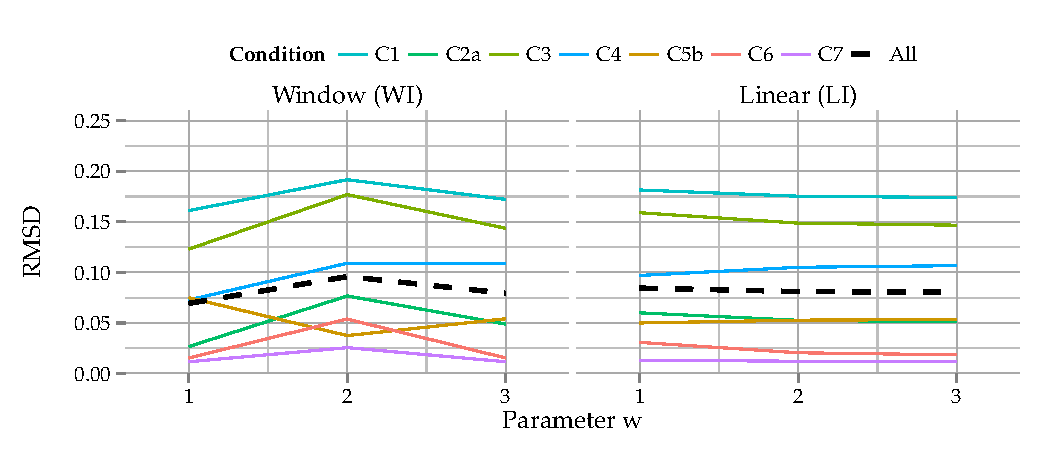
\includegraphics[width=\maxwidth]{figure/plotE1BASE-1} 

\end{knitrout}
	\caption[One session (\E1{}): multi-episodic prediction accuracy for the 3rd~usage episode (\acs{HP} only)]{One session (\E1{}): multi-episodic prediction accuracy for \ac{HP} only episodes (3rd usage episode).}
	\label{fig:pred:E1base}
\end{figure}

With regard to the multi\-/episodic judgment after the 6th~episode, both model types perform slightly differently.
\autoref{fig:pred:E1pred6} shows the \ac{RMSD} for the 6th~episode for both model types.
Here, WI performs better while increasing $\mathit{w}$ to 4 (0.23).
However, the prediction accuracy depends on the considered condition.
For example, \C3{} is far off for $\mathit{w}=1$ and improves until $\mathit{w}=3$, whereas \C4{} is best predicted with~$\mathit{w}=5$.
LI outperforms WI in prediction accuracy and is, furthermore, more robust.
For LI, the best accuracy is achieved for $\mathit{w}=2$.
All conditions except \C4{} and \C6{} yield here the minimal \ac{RMSD}.
In fact, \C4{} and \C6{} reach their minimum at~$\mathit{w}=3$.
Considering all conditions, the minimal \ac{RMSD} for LI is achieved at $\mathit{w}=2$ (0.12).
This is close to the prediction accuracy for presenting \ac{HP} episodes only.

\begin{figure}[b]
	\centering
\begin{knitrout}
\definecolor{shadecolor}{rgb}{0.969, 0.969, 0.969}\color{fgcolor}
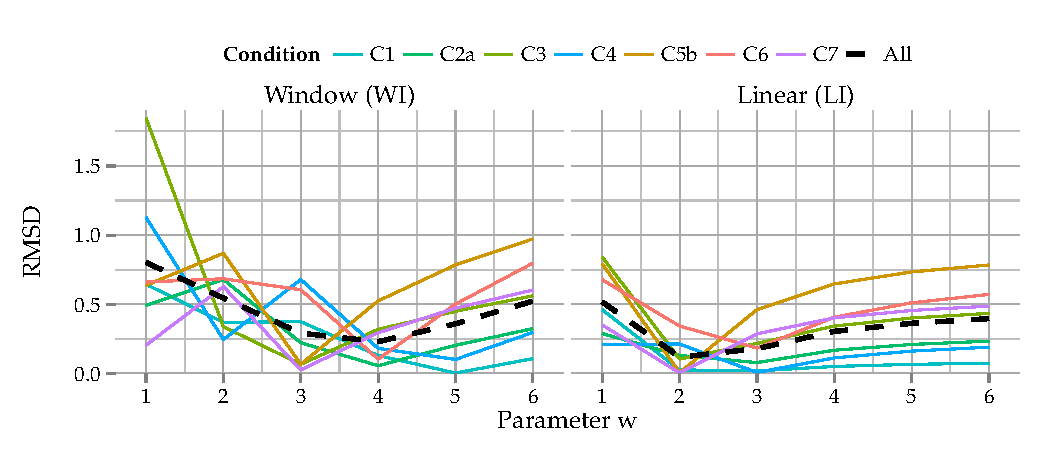
\includegraphics[width=\maxwidth]{figure/plotE1PRED-1} 

\end{knitrout}
	\caption[One session (\E1{}): multi-episodic prediction accuracy for the 6th~usage episode]{One session (\E1{}): multi-episodic prediction accuracy for all conditions (6th usage episode).}
	\label{fig:pred:E1pred6}
\end{figure}

With regard to the recovery (\autoref{hypo:recovery}), two conditions were investigated.
The \ac{RMSD} is shown for both weight functions in \autoref{fig:pred:E1pred9}.
WI is very precise for $\mathit{w}=4$ but is otherwise far off.
LI performs well for~\CVb{} with $\mathit{w} \geq 3$, whereas it performs very similarly for all $\mathit{w}$ in case of \C7{}.
Thus, LI is preferable, as it provides a higher robustness for the selection of $\mathit{w}$.

\begin{figure}[t]
	\centering
\begin{knitrout}
\definecolor{shadecolor}{rgb}{0.969, 0.969, 0.969}\color{fgcolor}
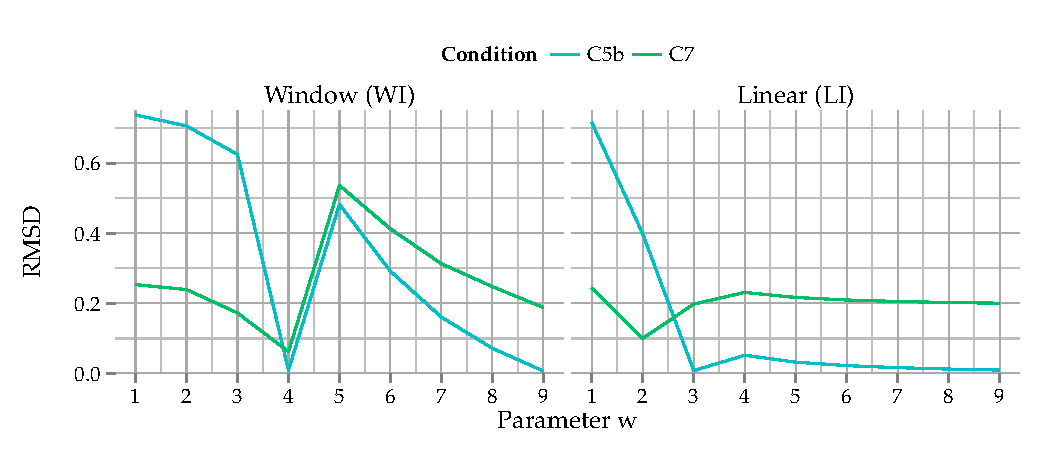
\includegraphics[width=\maxwidth]{figure/plotE1PRED9-1} 

\end{knitrout}
	\caption[One session (\E1{}): multi-episodic prediction accuracy for recovery]{One session (\E1{}): multi-episodic prediction accuracy for recovery (9th usage episode).}
	\label{fig:pred:E1pred9}
\end{figure}

\subparagraph*{Experiment E2a}
\EIIa{} complements \E1{} with a passive usage situation while it shares the performance levels.
With regard to the prediction of \ac{HP}-only episodes, the results are slightly different compared to \E1{}.
The prediction accuracy for the multi\-/episodic judgment after the 3rd~episode is shown in \autoref{fig:pred:E2pred3}.
Here, the prediction accuracy improves if $\mathit{w}$ is increased.
However, this is mainly due to~\C4{}.
The reason for this could not be determined.
Omitting \C4{} shows similar results compared to~\E1{}, \ie, the prediction accuracy is not affected by the selection of $\mathit{w}$.
The \ac{RMSD} is similar for all $\mathit{w}$ ($\textasciitilde 0.1$).
Here, no difference between~WI and~LI is observed.

\begin{figure}[b]
	\centering
\begin{knitrout}
\definecolor{shadecolor}{rgb}{0.969, 0.969, 0.969}\color{fgcolor}
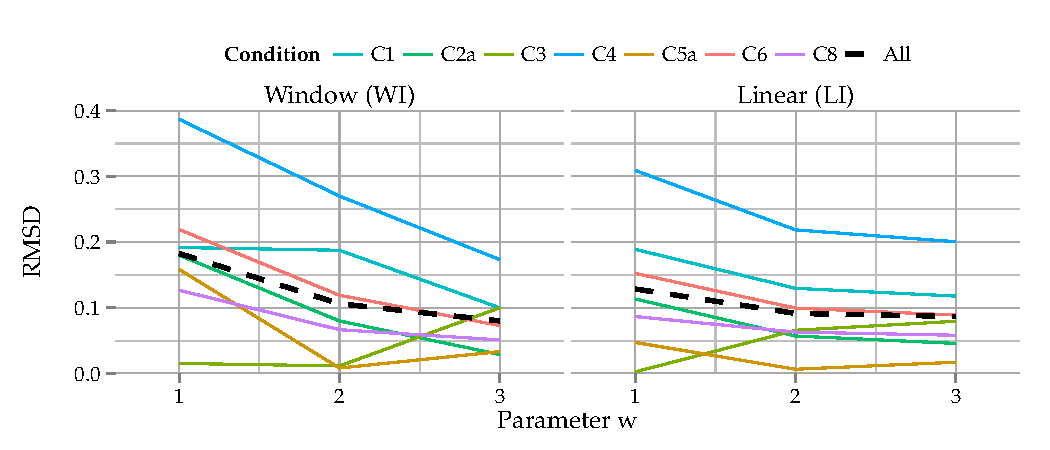
\includegraphics[width=\maxwidth]{figure/plotE2BASE-1} 

\end{knitrout}
	\caption[One session (\EIIa{}): multi-episodic prediction accuracy for the 3rd~usage episode (\acs{HP} only)]{One session (\EIIa{}): multi-episodic prediction accuracy for \acs{HP} only episodes (3rd~usage episode).}
	\label{fig:pred:E2pred3}
\end{figure}

With regard to the prediction of the multi\-/episodic judgment after the 6th~episode, the results closely resemble \E1{}.
The \ac{RMSD} is shown in \autoref{fig:pred:E2pred6}.
For WI, the minimal \ac{RMSD} is reached at $\mathit{w}=4$ (0.18) while $\mathit{w}=3$ (0.23) is rather close.
For LI, the minimal \ac{RMSD} is achieved at $\mathit{w}=2$ (0.13).
In fact, the found parameters are very similar to \E1{}, and the \ac{RMSD} behaves similarly for individual conditions.

\begin{figure}[h]
	\centering
\begin{knitrout}
\definecolor{shadecolor}{rgb}{0.969, 0.969, 0.969}\color{fgcolor}
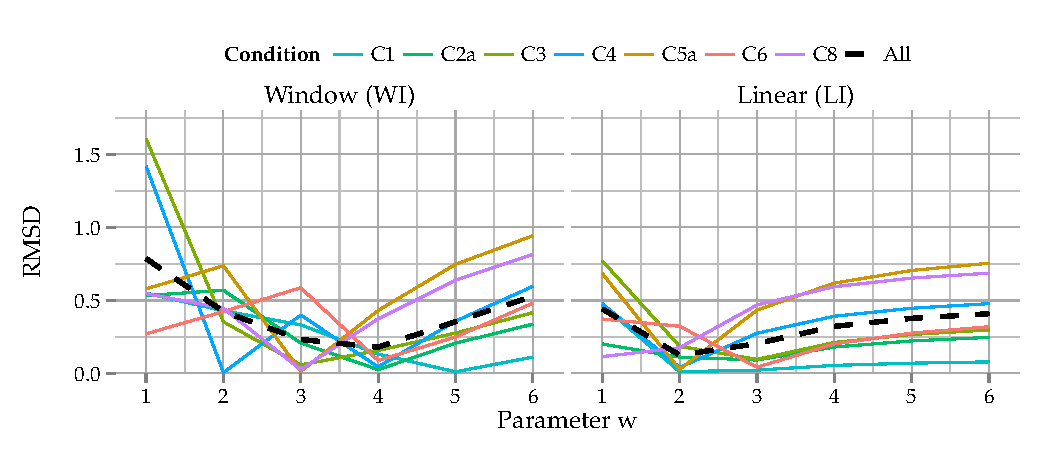
\includegraphics[width=\maxwidth]{figure/plotE2PRED-1} 

\end{knitrout}
 
	\caption[One session (\EIIa{}): multi-episodic prediction accuracy for the 6th~usage episode]{One session (\EIIa{}): multi-episodic prediction accuracy for all conditions (6th~usage episode).}
	\label{fig:pred:E2pred6}
\end{figure}

\subparagraph*{Conclusion}
For the prediction of multi\-/episodic judgments in one session, both weight functions perform similarly well.
For both experiments, it is notable that similar values for $\mathit{w}$ were found for each of the two weight functions.
With regard to the prediction accuracy, LI is preferable over~WI due to the better prediction accuracy.
Moreover, LI seems to be more robust against improper selection of $\mathit{w}$.
For both experiments, a minimal \ac{RMSD} could be achieved for $\mathit{w}=2$ in case of LI.
For the prediction of the multi\-/episodic judgment after the 9th~episode, which has only been investigated in \E1{}, LI ($\mathit{w}=3$) performs best. 
However, as only two conditions with regard to recovery were investigated (\autoref{hypo:recovery}), adjusting $\mathit{w}$ seems improper.

\subsection{Multiple Days: E6}
In \E6{}, a usage period of six~days was investigated for an \ac{AoD} service.
This service needed to be  used twice per day.
In this experiment, the first three~days (six~episodes) were presented in \ac{HP}.
Afterwards, the multi\-/episodic perceived quality was assessed.
Prediction accuracy for this judgment is shown in \autoref{fig:pred:E6pred6}.
Here, the prediction accuracy improves for an increasing $\mathit{w}$.
This is more prevalent for WI than for LI.
WI achieves its minimal \ac{RMSD} with $\mathit{w}=6$, \ie, all prior episodes.
LI provides only a marginal decrease for $\mathit{w} \geq 3$.

\begin{figure}[ht!]
	\centering
\begin{knitrout}
\definecolor{shadecolor}{rgb}{0.969, 0.969, 0.969}\color{fgcolor}
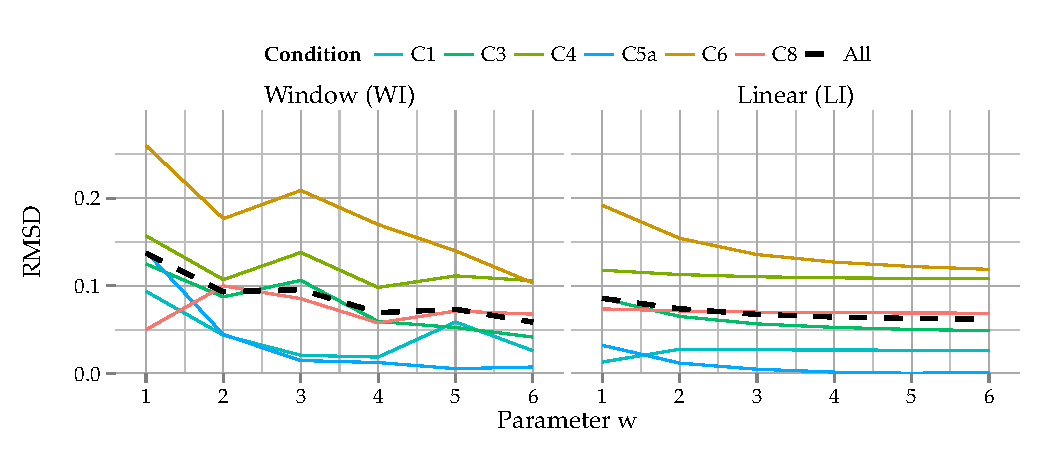
\includegraphics[width=\maxwidth]{figure/plotE6BASE-1} 

\end{knitrout}
	\caption[Multiple days (\E6{}): multi-episodic prediction accuracy after the 3rd~day (\acs{HP} only)]{Multiple days (\E6{}): multi-episodic prediction accuracy for \ac{HP} only episodes (3rd~day, \ie, 6th~usage episode).}
	\label{fig:pred:E6pred6}
\end{figure}

With regard to the prediction of the multi\-/episodic judgment of the 6th~day, both weight functions perform differently.
\autoref{fig:pred:E6pred12} shows the \ac{RMSD} for both weight functions.
While LI reaches a minimal \ac{RMSD} at $\mathit{w}=4$, WI achieves its minimal \ac{RMSD} not until $\mathit{w}=8$.
In addition, LI achieves a minimal \ac{RMSD} of 0.15, and WI only achieves a minimal \ac{RMSD} of
0.26.
With regard to \E6{}, LI is preferable to WI, as a higher prediction accuracy is achieved.
Furthermore, LI requires a smaller $\mathit{w}$ while it provides a higher robustness for choosing $\mathit{w}$.

\begin{figure}[b]
	\centering
\begin{knitrout}
\definecolor{shadecolor}{rgb}{0.969, 0.969, 0.969}\color{fgcolor}
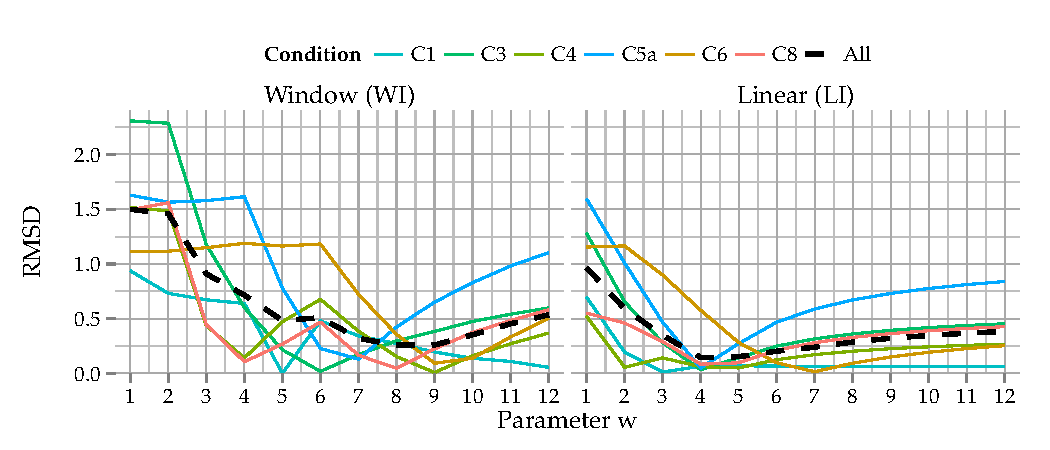
\includegraphics[width=\maxwidth]{figure/plotE6PRED-1} 

\end{knitrout}
	\caption[Multiple days (\E6{}): multi-episodic prediction accuracy after the 6th~day]{Multiple days (\E6{}): multi-episodic prediction accuracy for all conditions (6th~day, \ie, 12th~usage episode).}
	\label{fig:pred:E6pred12}
\end{figure}

\subsection{Saturation Effect}\label{pred:saturation}
In all three experiments, a saturation effect could be observed.
Here, the final multi\-/episodic judgment remained on the same level independent if two or three \ac{LP} episodes/days were presented, \ie, \C5{}\footnote{In the following, \C5{} refers to \CVb{} in case of \E1{} and to \CVa{} in case of \EIIa{}.
} and \C6{} were not judged differently.
In both cases, the multi\-/episodic judgment remained above the episodic judgments for \ac{LP} episodes (approx.~\unit[1]{pt}).
In fact, \C5{} and \C6{} only differ in the performance level of the 4th episode/day.
For \C5{}, this episode/day is presented in \ac{HP}, whereas \C6{} presented this episode/day in \ac{LP}.
As both conditions were not judged differently, this suggests that the difference in performance level of the 4th~episode/day does not seem to affect the formation process of the multi\-/episodic judgment.
%This implies that one \ac{LP} episode/day is not judged differently than one \ac{HP} episode with regard to the multi\-/episodic judgment.
%This can be modeled in two ways.
%On the one hand, the weight of one of the three \ac{LP} episodes/days can be set to zero, and the weight of \ac{HP} episodes increased.
%
%The later would be necessary due to the reduced number of \ac{HP} episodes.
%On the other hand, the episodic judgment of one \ac{LP} episode/day can be adjusted.
%Here, the episodic judgment(s) of this episode/day would be changed to a \ac{HP}.
%This omits adjusting the weight function to cover this effect.
%The second option seems more elegant and is more likely to reflect a characteristic of the quality formation process.
%It must be noted that the multi-episodic judgments remain above the episodic judgments for \ac{LP} episodes.
%It is thus concluded that in this case one of the three \ac{LP} episodes did not attribute to the multi\-/episodic judgment.
%One option to enhance the prediction model is to adjust the weight function to decrease the weight of one or more \ac{LP} episode(s) and increase the weight of one or more \ac{HP} episode(s).
%The later is necessary to compensate for the lack of one \ac{HP} usage episodes/day.
With regard to the applicability of the weighted average, this is problematic, as a model needs to produce a similar prediction based on different inputs, \ie, one \ac{HP} episode/day and two \ac{LP} episodes/days (\C5{}) versus three \ac{LP} episodes/days (\C6{}).
As the multi-episodic judgment remained above the level of episodic judgments of \ac{LP} episodes, at least the last four episodes/days must be considered in the case of \C6{}, whereas \C5{} only requires at least three episodes/days.
For all three experiments, LI and WI require a larger $\mathit{w}$ to reach the best prediction accuracy for \C6{} compared to all other conditions.
For \E1{} and \EIIa{}, $\mathit{w}=3$~(LI) and $\mathit{w}=4$~(WI) are required for \C6{}, whereas \C5{} achieves its lowest prediction accuracy already at $\mathit{w}=2$~(LI) and $\mathit{w}=3$~(WI).
For \E6{}, $\mathit{w}=7$~(LI) and $\mathit{w}=9$~(WI) are required for \C6{}, whereas \C5{} achieves its lowest prediction error at $\mathit{w}=4$~(LI) and $\mathit{w}=7$~(WI).
It must be noted that the optimal value(s) of $\mathit{w}$ for LI as well as WI in case of \C5{} are identical to the optimal $\mathit{w}$ for all conditions.
Thus, the overall prediction performance for both weight functions can be improved if $\mathit{w}$ can be reduced to this value in case of \C6{}.
Although the underlying reason for the observed saturation effect could not be deduced, this can be achieved by \emph{modifying} the episodic judgment(s) of the 4th~episode/day for \C6{}, so it resembles \C5{}.
This modification can be achieved by replacing these judgment(s) by the average of episodic judgments of \ac{HP} episodes. 
%However, a simpler approach can be derived by assuming that one of the \ac{LP} usage episodes/days did not only not contribute to the multi\-/episodic judgment, but rather is considered as \ac{HP} for the judgment of multi\-/episodic perceived quality, \ie, that \C5{} and \C6{} are not considered differently with regard to the formation process.
It is thus here proposed to change $\mathit{e_4}$ in case of \C6{} for \E1{} and \EIIa{}:
\begin{equation}\label{eq:saturate:modify1}
\tilde{e}_4=\nicefrac{1}{3} \sum\limits_{i=1}^{3}e_i \, .
\end{equation}
For \E6{}, the episodic judgments of $\mathit{e_7}$ and $\mathit{e_8}$ are adjusted as follows:
\begin{equation}\label{eq:saturate:modify2}
\tilde{e}_{[7,8]}= \nicefrac{1}{6} \sum\limits_{i=1}^{6}e_i \, .
\end{equation}
This is equivalent to extending $\mathit{\hat{m}_n}$ in the case of \C6{} with the addition of the term (here only shown for \E1{} and \EIIa{}):
\begin{equation}\label{eq:saturate:addition}
(\nicefrac{\sum\limits_{i=1}^{3}e_i}{3} - e_4) \cdot  \nicefrac{a_4}{\sum\limits_{i=1}^{n}a_i}\, .
\end{equation}

This modified version of \C6{} is denoted as \emph{\C6{}~(adjusted)}.
In the following, the prediction accuracy of the two weight functions for \C5{}, \C6{}, and \C6{}~(adjusted) is presented.
For \E1{} and \EIIa{}, this is shown in \autoref{fig:pred:SAT:E1} and \autoref{fig:pred:SAT:E2a}, respectively.

\begin{figure}
	\centering
\begin{knitrout}
\definecolor{shadecolor}{rgb}{0.969, 0.969, 0.969}\color{fgcolor}
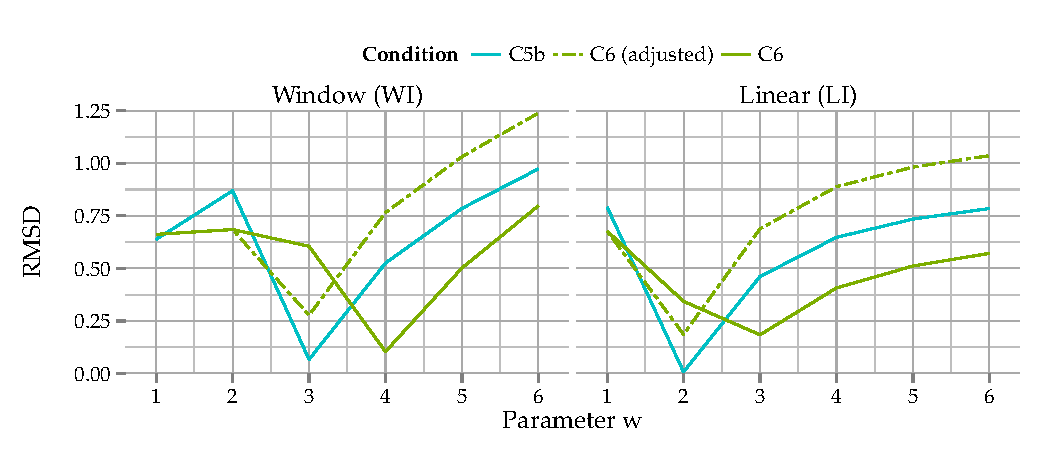
\includegraphics[width=\maxwidth]{figure/plotE1SAT-1} 

\end{knitrout}
	\caption[One session (\E1{}): multi-episodic prediction accuracy for the saturation effect]{One session (\E1{}):  multi-episodic prediction accuracy for saturation effect (6th~usage episode).}
	\label{fig:pred:SAT:E1}
\end{figure}

For \E1{} and \EIIa{}, this adjustment results in a shift of the minimal \ac{RMSD} for the two weight functions.
In case of WI, the minimal \ac{RMSD} shifts from~$\mathit{w}=4$ to~$\mathit{w}=3$ for both experiments.
This is also observed for LI.
Here, the minimal \ac{RMSD} shifts from~$\mathit{w}=3$ to~$\mathit{w}=2$.
It is notable for both experiments that this adjustment leads to a similar shape of \ac{RMSD} in case of \C5{} and \C6{}~(adjusted).
Furthermore, the minimal \ac{RMSD} is reached earlier, but for increasing $\mathit{w}$ the \ac{RMSD} is worse for \C6{}~(adjusted) than for \C6{}.
\begin{figure}
	\centering
\begin{knitrout}
\definecolor{shadecolor}{rgb}{0.969, 0.969, 0.969}\color{fgcolor}
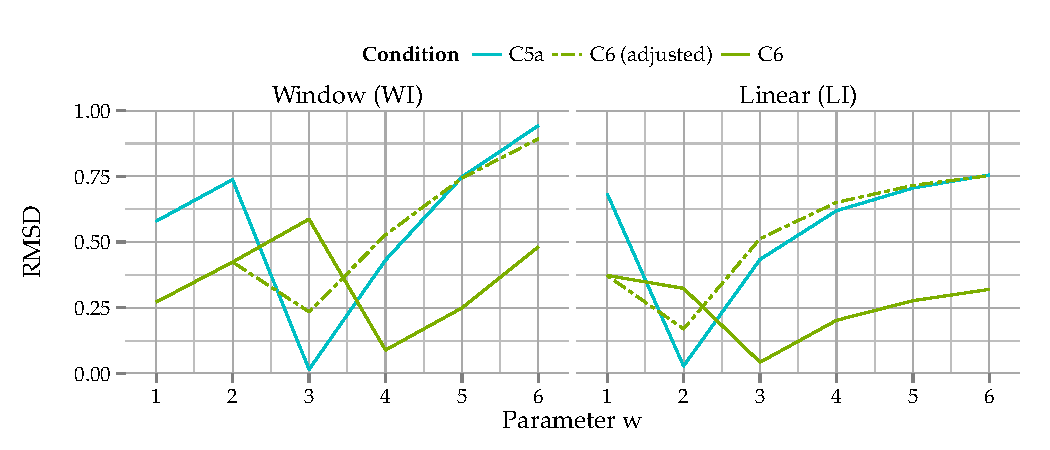
\includegraphics[width=\maxwidth]{figure/plotE2SAT-1} 

\end{knitrout}
	\caption[One session (\EIIa{}):  multi-episodic prediction accuracy for the saturation effect]{One session (\EIIa{}):  multi-episodic prediction accuracy for the saturation effect (6th~usage episode).}
	\label{fig:pred:SAT:E2a}
\end{figure}

With regard to \E6{}, a similar observation is made.
The minimal \ac{RMSD} shifts from $\mathit{w}=9$~to~ $\mathit{w}=6$ for WI and for LI from $\mathit{w}=7$ to $\mathit{w}=4$.
Here, \C6{}~(adjusted) also resembles \C5{} closely (see \autoref{fig:pred:SAT:E6}).

\begin{figure}
	\centering
\begin{knitrout}
\definecolor{shadecolor}{rgb}{0.969, 0.969, 0.969}\color{fgcolor}
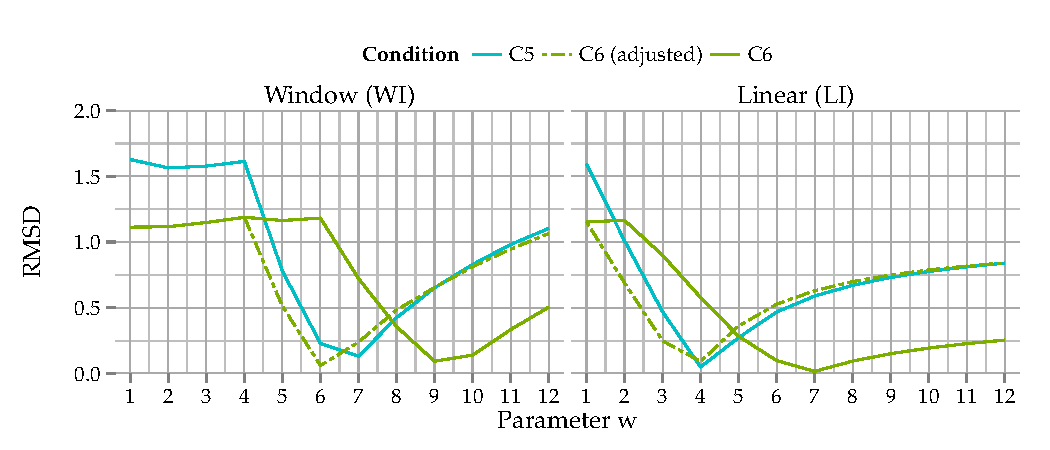
\includegraphics[width=\maxwidth]{figure/plotE6SAT-1} 

\end{knitrout}
	\caption[Multiple days (\E6{}):  multi-episodic prediction accuracy for the saturation effect]{Multiple days (\E6{}):  multi-episodic prediction accuracy for the saturation effect (6th~day, \ie, 12th~usage episode).}
	\label{fig:pred:SAT:E6}
\end{figure}

It can thus be concluded that the saturation effect can be accounted for by using the proposed algorithm.
For all three experiments, this algorithm resulted in a reduction of $\mathit{w}$.
%In fact, $\mathit{w}$ is reduced to the optimal found solution for each experiment, when evaluating all conditions (see \autoref{results:prediction}).
Although the \ac{RMSD} is increased in some cases, $\mathit{w}$ is reduced to the optimal solution considering all conditions without the saturation adjustment (see \autoref{results:prediction}).
For all conditions, applying the adjustment leads to a reduction of the \ac{RMSD} (\E1{}: 0.02, \EIIa{}: 0.03, and \E6{}: 0.08).
In fact, this overall reduction is rather small with regard to all conditions.

%round(min(subset(data_mos_nonadjusted, data_mos_nonadjusted[["experiment"]] == "E6a" & data_mos_nonadjusted[["id"]] == 14 & data_mos_nonadjusted[["model"]] == "weight_linear_create" & data_mos_nonadjusted[["condition"]] == "All")[["RMSD"]]), 2)
%round(min(subset(data_mos_adjusted, data_mos_adjusted[["experiment"]] == "E6a" & data_mos_adjusted[["id"]] == 14 & data_mos_adjusted[["model"]] == "weight_linear_create" & data_mos_adjusted[["condition"]] == "All")[["RMSD"]]), 2)

%round(min(subset(data_mos_nonadjusted, data_mos_nonadjusted[["experiment"]] == "E1" & data_mos_nonadjusted[["id"]] == 6 & data_mos_nonadjusted[["model"]] == "weight_linear_create" & data_mos_nonadjusted[["condition"]] == "All")[["RMSD"]]), 2)
%round(min(subset(data_mos_adjusted, data_mos_adjusted[["experiment"]] == "E1" & data_mos_adjusted[["id"]] == 6 & data_mos_adjusted[["model"]] == "weight_linear_create" & data_mos_adjusted[["condition"]] == "All")[["RMSD"]]), 2)

%round(min(subset(data_mos_nonadjusted, data_mos_nonadjusted[["experiment"]] == "E2a" & data_mos_nonadjusted[["id"]] == 6 & data_mos_nonadjusted[["model"]] == "weight_linear_create" & data_mos_nonadjusted[["condition"]] == "All")[["RMSD"]]), 2)
%round(min(subset(data_mos_adjusted, data_mos_adjusted[["experiment"]] == "E2a" & data_mos_adjusted[["id"]] == 6 & data_mos_adjusted[["model"]] == "weight_linear_create" & data_mos_adjusted[["condition"]] == "All")[["RMSD"]]), 2)


\section{Conclusion}
In this chapter, two model types based on the weighted average for predicting the multi\-/episodic \ac{MOS} using the episodic \ac{MOS} were presented.
It could be shown that a weighted average using either a window function or a linear function enabled to predict the multi\-/episodic \ac{MOS}.
Both weight functions perform similarly if only \ac{HP} usage episodes were presented.
In fact, if \ac{LP} usages episodes were presented, both outperform the unweighted average of all prior episodic judgments, \ie, a smaller $\mathit{w}$ achieves a better prediction accuracy.
Comparing WI and LI, the latter shows a better prediction accuracy and higher robustness for choosing the $\mathit{w}$.
This is observed in all three experiments.
One interesting observation is made with regard to the one-session experiments.
For both weight functions, the highest prediction accuracy is achieved for the same $\mathit{w}$ in case of \E1{} and \EIIa{}, \ie, LI:~$\mathit{w}=2$ and WI:~$\mathit{w}=4$.
This suggests that the usage situation must actually not be considered in this case for predicting the multi\-/episodic \ac{MOS}.

Although no reason for the observed saturation effect could be derived, accounting for it with the described algorithm improves the overall prediction accuracy for all three experiments.

In fact, it must be noted that the weighted average with the rather simple weight functions (one degree of freedom) enabled a decent prediction accuracy for one session as well as a usage period of 6~days.
Nevertheless, the conducted modeling is inherently limited to the data of the conducted experiments, and models could not be verified as no data sets were available that could be used for cross\-/validation.
